\section{Funciones continuas}
Sea $f:D \subset \mathbb{R}^n \to \mathbb{R}^m$. Se dice que $f$ es \textbf{continua} en un punto $X_0 \in D$ si:
\begin{itemize}
    \item $\exists \lim_{X \to X_0} f(X) = L$
    \item $f(X_0) = L$
\end{itemize}

\begin{nota}[colback=blue!5,colframe=blue!60, title=Definiciones]
\begin{itemize}
    \item Se dice que $f$ es continua en un subconjunto $S \subset D$ si es 
    continua en todos los puntos de $S$.
    \item Se dice que $f$ es continua si es continua en todo su dominio.
\end{itemize}
\end{nota}

\begin{nota}[colback=yellow!5,colframe=yellow!80, title=Importante]
La suma, resta, producto y división (cuando el denominador no es cero) de funciones continuas
es continua.
\end{nota}

\subsection{Teoremas de continuidad}

\subsubsection{Teorema I: composición de funciones continuas}
Sea $f:D \subset \mathbb{R}^n \to \mathbb{R}^m$ y $g:E \subset \mathbb{R}^m \to \mathbb{R}^p$ y supongamos que
$f(D) \subset E$. Si $f$ es continua en $X_0 \in D$ y $g$ es continua en
$f(X_0) \in E$, entonces la función compuesta $g \circ f:D \to \mathbb{R}^p$, definida por 
$h(X) = (g \circ f)(X) = g(f(X))$ es continua en $X_0$.

\begin{figure}[H] 
    \centering    
    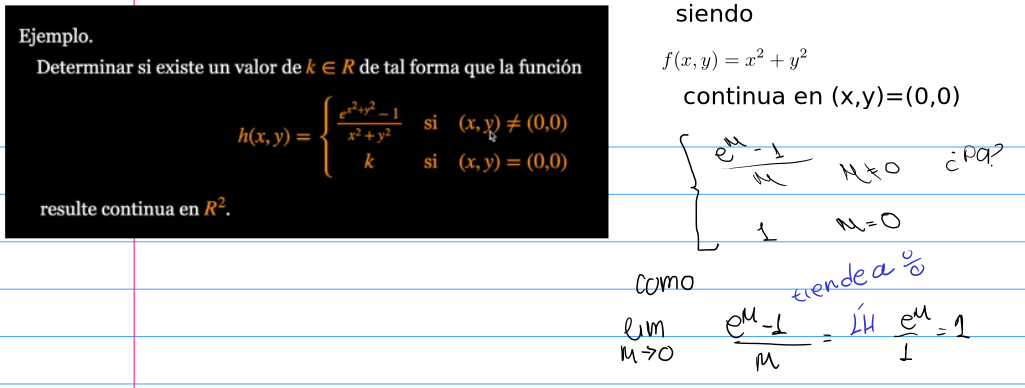
\includegraphics[width=0.8\textwidth]{img/ej-cont.png}
    \label{fig:ej-cont}
\end{figure}

\subsubsection{Teorema I: curvas}

\begin{itemize}
    \item Sea $f:   \mathbb{R}^n \to \mathbb{R}^m$ una función continua y $C \subset \mathbb{R}^n$ un conjunto conexo.
    Entonces el conjunto $f(C) \subset \mathbb{R}^m$ es conexo.
    \item Sea $f:\mathbb{R}^n \to \mathbb{R}^m$ una función continua y $C \subset \mathbb{R}^n$ un conjunto compacto.
    Entonces el conjunto $f(C) \subset \mathbb{R}^m$ es compacto.
\end{itemize}

\begin{nota}[colback=green!5,colframe=green!80, title=Definición importante]
Sea $\vec{g}: I \subset \mathbb{R} \to \mathbb{R}^n$. Entonces si 
$
\begin{cases}
    I \text{ es un intervalo} \\
    \vec{g} \text{ es continua en } I
\end{cases}
$ 
al conjunto imagen de $\vec{g}$ se lo llamará \textbf{curva continua} en $R^n$.
\end{nota}

\begin{figure}[H] 
    \centering    
    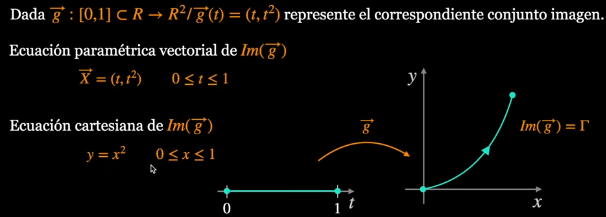
\includegraphics[width=0.7\textwidth]{img/ej-curva.png}
    \label{fig:ej-curva}
\end{figure}
\begin{figure}[H] 
    \centering    
    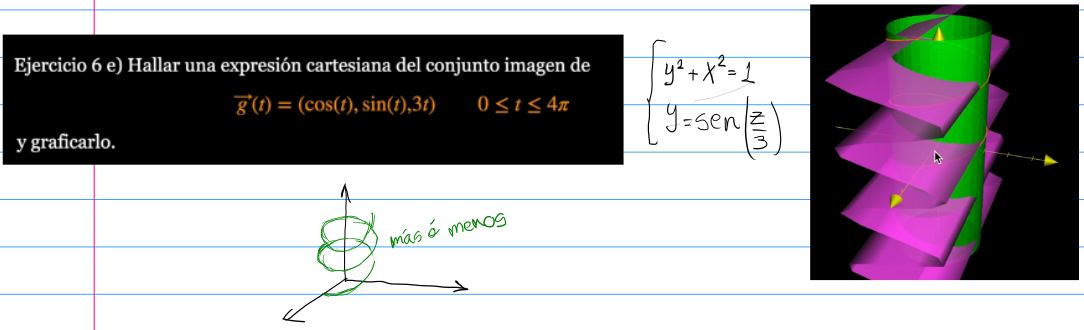
\includegraphics[width=0.8\textwidth]{img/ej-curva2.png}
    \label{fig:ej-curva2}
\end{figure}


\begin{nota}[colback=blue!5,colframe=blue!60, title=Definiciones]
Dada una curva $C \subset \mathbb{R}^m$ de ecuación $\vec{X}=\vec{g}(t)$ definimos:
\begin{itemize}
    \item Un punto $A = \vec{g}(t_0)$ es un \textbf{punto regular} de la curva
    cuando $\vec{g}$ es derivable en $t_0$ y $\vec{g}'(t_0) \neq 0$. Una curva es
    \textbf{regular} si todos sus puntos son regulares.

    \item Un punto $A = \vec{g}(t_0)$ es un \textbf{punto simple} de la curva cuando,
    a través de $\vec{g}$, es imagen de un único valor de $t_0 \in I$. 
    Una curva es \textbf{simple} si todos sus puntos son simples.

    \item  Un \textbf{arco de curva} es una curva de ecuación $\vec{X}=\vec{g}(t)$ con $t \in [a,b]$,
    en el intervalo $I$ cerrado y acotado. Si además $\vec{g}(a) = \vec{g}(b)$ diremos que el arco de curva es cerrado.
    Un arco de curva cerrado es simple si lo es la curva de ecuación $\vec{X}=\vec{g}(t)$ con $t \in [a,b)$.
\end{itemize}
\end{nota}

\begin{figure}[H] 
    \centering    
    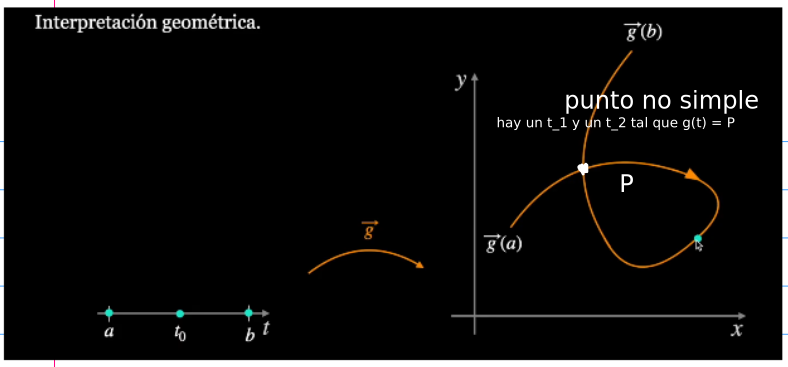
\includegraphics[width=0.8\textwidth]{img/ej-curva3.png}
    \label{fig:ej-curva3}
\end{figure}